\chapter{State of the art}
This chapter is about the state of the art.

\section{Theory}
This section is about the theory, for example dynamics and underactuated control.

\subsection{Underactuated system}
According to Newtons second law(\( F = ma \)), The dynamics of mechanical systems can be discribed as follows:
\begin{align}
    \ddot{q} = f(q, \dot{q}, u, t)
\end{align}

Where the state is given by a vector of positions(also known as the configuration vector), and a vector of velocities, \( \dot{q}\).

For control, the second order differential equation can be rewritten as below:

\begin{align}
    \ddot{q} = f_1(q, \dot{q}, t) + f_2(q, \dot{q}, t)u
\end{align}

For a controlled dynamical system described by equation(2.2), if we have:

\begin{align}
    \text{rank}[f_2(q, \dot{q}, t)] < \text{dim}[q]
\end{align}

then the system is underactuated at \((q, \dot{q}, t)\)\cite{tedrake2022underactuated}. There is another case for underactuation is even when \(f_2\) is full rank, but additional constraints like \(|\mathbf{u}| \leq 1\) can also make a system underactuated.


\subsection{Dynamics of underactuated double pendulum system}
As shown in figure 2.1, we model the dynamics of the double pendulum with 15 parameters which include 8 link parameters namely masses \((m_1,m_2)\)
, lengths \((l_1,l_2)\)
, center of masses \((r_1,r_2)\) 
, inertias \((I_1,I_2)\)
 for the two links, and 6 actuator parameters namely motor inertia \(I_r\)
, gear ratio \(g_r\)
, coulomb friction \((c_{f1},c_{f2})\)
, viscous friction \((b_1,b_2)\)
 for the two joints and gravity.
\begin{figure}[h]
  \centering
  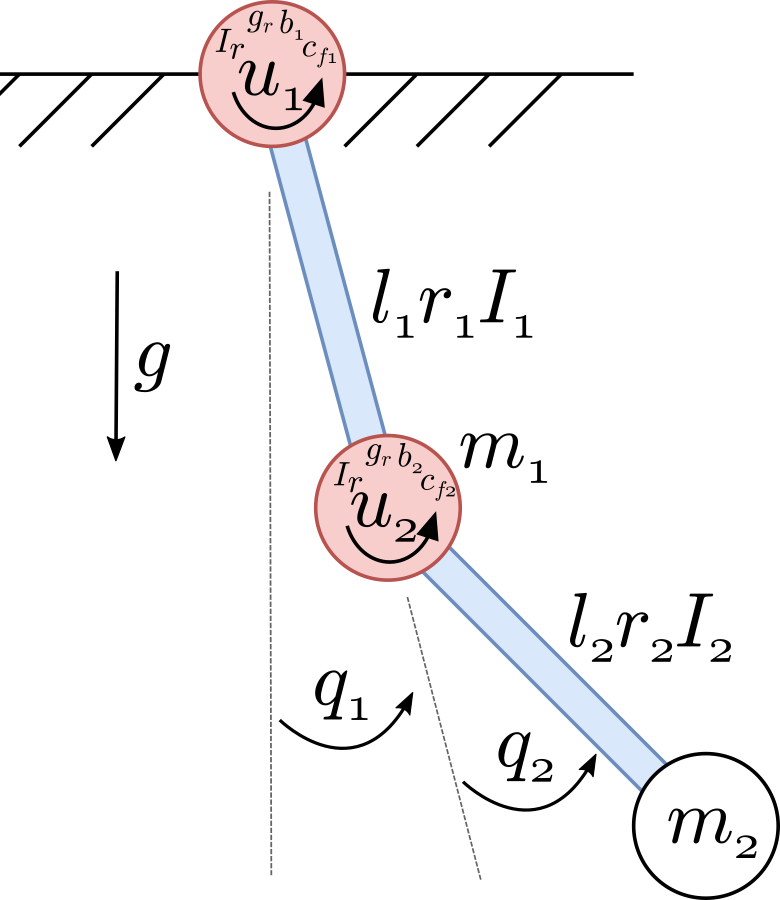
\includegraphics[width=0.5\textwidth]{figures/double_pendulum_dynamics.png} % Replace "example-image" with the actual image file name and path
  \caption{Double pendulum dynamics}
  \label{fig:sample}
\end{figure}

The generalized coordinates \( \mathbf{q} =(q_1,q_2)^T \) are the joint angles measured from the free hanging position. The state vector of the systems contains the position coordinates and their time derivatives: \(\mathbf{x}=(\mathbf{q},\mathbf{\dot{q}})^T\). The torque applied by the actuators are \(\mathbf{u}=(u_1,u_2)\). The equation of motion for the dynamics of a dynamical system can be derived following the blow steps:

\textbf{Step 1. Define the Lagrangian (\(L\)):}

   The Lagrangian (\(L\)) is defined as the difference between the kinetic energy (\(T\)) and the potential energy (\(U\)) of the system:
   \begin{align}
         L = T - U
   \end{align}


\textbf{Step 2. Express the Kinetic Energy (\(T\)):}

   The kinetic energy (\(T\)) of the double pendulum is the sum of the kinetic energies of both links. The kinetic energy for a link is given by:
   \begin{align}
        T = \frac{1}{2} m_1 (\dot{x}_1^2 + \dot{y}_1^2) + \frac{1}{2} m_2 (\dot{x}_2^2 + \dot{y}_2^2)
   \end{align}

   where \(m_1\) and \(m_2\) are the masses of the links, \((x_1, y_1)\) and \((x_2, y_2)\) are their positions, and \(\dot{x}_1, \dot{y}_1, \dot{x}_2, \dot{y}_2\) are their respective velocities.

\textbf{Step 3. Express the Potential Energy (\(U\)):}

   The potential energy (\(U\)) of the double pendulum is the sum of the potential energies of both links. The potential energy for a link in a gravitational field is given by:
   \begin{align}
         U = m_1 g y_1 + m_2 g y_2
   \end{align}

   where \(g\) is the acceleration due to gravity.
   
   
\textbf{Step 4. Formulate the Lagrange's Equation:}

   Use Lagrange's equation to derive the equations of motion for the generalized coordinates \(x_1, y_1, x_2, y_2\).

    \begin{align}
    \frac{d}{dt} \left(\frac{\partial L}{\partial \dot{q_i}}\right) - \frac{\partial L}{\partial q_i} = 0
    \end{align}

\textbf{Step 5. Solve the Equations of Motion:}

   Solve the obtained set of second-order differential equations to determine the equations of motion for the system. The system dynamics with friction is:
   
   \begin{align}
        M(q)\ddot{q} + C(q,\dot{q})\dot{q} &= Du + G(q) - F(\dot{q})
   \end{align}
    
    Because the state vector is \(\mathbf{x}=(\mathbf{q},\mathbf{\dot{q}})^T\), the equation of motion can also be expressed as:
    
    \begin{equation}
    \begin{split}
        \dot{x} &= f(x,u) \\
        &= \begin{bmatrix} 
            \dot{q} \\ 
            M^{-1}(Du - C(q,\dot{q})\dot{q} + G(q) - F(\dot{q})) 
       \end{bmatrix}
    \end{split}
    \end{equation}

   Consider the forward kinematics of double pendulum system, the coordinate of the joint between the first link and the second link is \(P_1=(x_1,y_1)\),the coordinate of the end effector is \(P_2=(x_2,y_2)\).

    \begin{align}
        \label{eq:first_set}
        \left\{
        \begin{aligned}
        x_1 &= l_1 \sin(q_1) \\
        y_1 &= - l_1 \cos(q_1)
        \end{aligned}
        \right.
    \end{align}

    \begin{align}
        \label{eq:second_set}
        \left\{
        \begin{aligned}
        x_2 &= l_1 \sin(q_1) + l_2 \sin(q_1 + q_2) \\
        y_2 &= -l_1 \cos(q_1) - l_2 \cos(q_1 + q_2)
        \end{aligned}
        \right.
    \end{align}

    Put equation(2.10) and (2.11) into (2.6)(2.7)(2.8)(2.9),we can get the mass matrix (with \(s_1 = \sin(q_1), c_1 = \cos(q_1), \ldots\))
    \begin{equation}
    \mathbf{M} =
    \left[ 
    {\begin{array}{cc}
    I_1 + I_2 + l_1^2m_2 + 2l_1m_2r_2c_2 + g_r^2I_r + I_r  &   I_2 + l_1m_2r_2c_2 - g_rI_r  \\
    I_2 + l_1m_2r_2c_2 - g_rI_r                    & I_2 + g_r^2I_r                       \\
    \end{array}} 
    \right]
    \end{equation}
    
    the Coriolis matrix:
    \begin{equation}
    \begin{split}
    \mathbf{C} = \left[
    \begin{matrix}
    -2 \dot{q}_2 l_{1} m_{2} r_{2} \sin(q_2) & -\dot{q}_2 l_{1} m_{2} r_{2} \sin(q_2)\\
    \dot{q}_1 l_{1} m_{2} r_{2} \sin(q_2) & 0
    \end{matrix}
    \right],
    \label{eq:coriolis_matrix}
    \end{split}
    \end{equation}
    
    The gravity vector:
    \begin{equation}
    \begin{split}
    \mathbf{G} = \left[
    \begin{matrix}
    - g m_{1} r_{1} \sin(q_1) - g m_{2} \left(l_{1} \sin(q_1) + r_{2} \sin(q_{1+2}) \right) \\
    - g m_{2} r_{2} \sin(q_{1+2})
    \end{matrix}
    \right],
    \label{eq:gravity_matrix}
    \end{split}
    \end{equation}
    
    The friction vector:
    \begin{equation}
        \begin{split}
            \mathbf{F} =
            \left[
                \begin{matrix}
                    b_1 \dot{q}_1 + c_{f1} \arctan(100\,\dot{q}_1) \\
                    b_2 \dot{q}_2 + c_{f2} \arctan(100\,\dot{q}_2)
                \end{matrix}
            \right]
        \end{split}
    \end{equation}
    (the \(\arctan(100\,\dot{q}_i)\) function is used to approximate the discrete step function for the coulomb friction)

    and the actuator selection matrix \(\mathbf{D}\):
    \begin{equation}
        \begin{split}
            \mathbf{D}_{full} =
            \left[
                \begin{matrix}
                    1 & 0 \\
                    0 & 1
                \end{matrix}
            \right],
            \quad
            \mathbf{D}_{pendu} =
            \left[
                \begin{matrix}
                    1 & 0 \\
                    0 & 0
                \end{matrix}
            \right],
            \quad
            \mathbf{D}_{acro} =
            \left[
                \begin{matrix}
                    0 & 0 \\
                    0 & 1
                \end{matrix}
            \right]
        \end{split}
    \end{equation}
    for the fully actuated system, the pendubot or the acrobot.

\section{Related work}
In this section, we want to introduce the methods of underactuated control and the works related.

Extensive research has been conducted on complex robotic motion control, with learning-based methods gaining widespread adoption in recent times. 

A notable example is the classical control module within the Gymnasium environment, a well-known reinforcement learning framework developed by OpenAI. This module serves as an ideal platform for exploring and evaluating new motion control algorithms. 

Another noteworthy achievement in the field is the DeepMimic project [2]. Through imitation learning within a simulated environment, this project has enabled robots to acquire intricate human movements, including backflips and martial arts maneuvers. 

Additionally, a research team from ETH Zurich has made significant progress in addressing the sim-to-real interface challenge [3]. Their methodology involves training a control model for a mini-cheetah-like robot within a simulation environment. By utilizing a neural network and leveraging data collected from the real robot, they approximated the dynamics model of the physical robot. This approach has facilitated accurate implementation of the control policy derived from the virtual environment onto the real robot. These exemplary works demonstrate the promising applications of learning-based approaches in various aspects of robot control.

\cleardoublepage
